%%%%%%%%%%%%%%%%%%%%%%%%%%%%%%%%%%%%%%%%%%%%%%%%%%%%%%%%%%%%%%%%%%%%%%%%%%%%%%%%%%
\begin{frame}[fragile]\frametitle{}
\begin{center}
{\Large Natural Language Processing: An Introduction}
\end{center}
\end{frame}

%%%%%%%%%%%%%%%%%%%%%%%%%%%%%%%%%%%%%%%%%%%%%%%%%%%%%%%%%%%%%%%%%%%%%%%%%%%%%%%%%%
\begin{frame}[fragile]\frametitle{}
\begin{center}
{\Large Background: What is Language?}
\end{center}
\end{frame}


%%%%%%%%%%%%%%%%%%%%%%%%%%%%%%%%%%%%%%%%%%%%%%%%%%%%%%%%%%%%%%%%%%%%%%%%%%%%%%%%%%
\begin{frame}[fragile]\frametitle{xkcd}
\begin{center}
\includegraphics[width=\linewidth,keepaspectratio]{nlpxkcd}
\end{center}

{\tiny (Parables: verse/short stories with morals)}
\end{frame}


%%%%%%%%%%%%%%%%%%%%%%%%%%%%%%%%%%%%%%%%%%%%%%%%%%%%%%%%%%%%%%%%%%%%%%%%%%%%%%%%%%
\begin{frame}[fragile]\frametitle{What's a Language?}
\begin{center}
\includegraphics[width=0.8\linewidth,keepaspectratio]{nlp_basics}
\end{center}
\end{frame}

%%%%%%%%%%%%%%%%%%%%%%%%%%%%%%%%%%%%%%%%%%%%%%%%%%%%%%%%%%%%%%%%%%%%%%%%%%%%%%%%%%
\begin{frame}[fragile]\frametitle{What's a Language?}
\begin{center}
\includegraphics[width=0.8\linewidth,keepaspectratio]{not_all}
\end{center}
\end{frame}



%%%%%%%%%%%%%%%%%%%%%%%%%%%%%%%%%%%%%%%%%%%%%%%%%%%%%%%%%%%%%%%%%%%%%%%%%%%%%%%%%%
\begin{frame}[fragile] \frametitle{$Words == Meaning$?}
 \begin{center}
When you read the word, say, ``Crab'', what does this mean to you?



Bunch of letters? or something else?
\end{center}
\end{frame}

%%%%%%%%%%%%%%%%%%%%%%%%%%%%%%%%%%%%%%%%%%%%%%%%%%%%%%%%%%%%%%%%%%%%%%%%%%%%%%%%%%
\begin{frame}[fragile] \frametitle{$Words == Meaning$?}
\begin{center}
\includegraphics[width=0.8\linewidth,keepaspectratio]{crab1}
\end{center}
Is the symbol representative of its meaning? 
\end{frame}


%%%%%%%%%%%%%%%%%%%%%%%%%%%%%%%%%%%%%%%%%%%%%%%%%%%%%%%%%%%%%%%%%%%%%%%%%%%%%%%%%%
\begin{frame}[fragile] \frametitle{$Words == Meaning$?}
Now, which of these you can understand?

\begin{center}
\includegraphics[width=0.8\linewidth,keepaspectratio]{crab2}
\end{center}
Or is it just a mapping in a mental lexicon/vocabulary/dictionary (word, picture, understanding)?
\end{frame}

% %%%%%%%%%%%%%%%%%%%%%%%%%%%%%%%%%%%%%%%%%%%%%%%%%%%%%%%%%%%%%%%%%%%%%%%%%%%%%%%%%%
% \begin{frame}[fragile]\frametitle{Words and Meaning}
% When you read the word "Crab", what does this mean to you?
% \begin{center}
% \includegraphics[width=0.6\linewidth,keepaspectratio]{crab1}
% \end{center}

% Is the symbol representative of its meaning?

% Or just arbitrary mapping in mental lexicon?
% \begin{center}
% \includegraphics[width=0.6\linewidth,keepaspectratio]{crab2}
% \end{center}
% \end{frame}

%%%%%%%%%%%%%%%%%%%%%%%%%%%%%%%%%%%%%%%%%%%%%%%%%%%%%%%%%%%%%%%%%%%%%%%%%%%%%%%%%%
\begin{frame}[fragile]\frametitle{Arbitrariness of Language Symbols}
\begin{center}
\includegraphics[width=0.6\linewidth,keepaspectratio]{crab3}
\end{center}

These symbols are arbitrary. Words don't embed knowledge by themselves.

But words are the only thing we have for processing!

Verbal and written communication is primarily through words.
\end{frame}

%%%%%%%%%%%%%%%%%%%%%%%%%%%%%%%%%%%%%%%%%%%%%%%%%%%%%%%%%%%%%%%%%%%%%%%%%%%%%%%%%%
\begin{frame}[fragile]\frametitle{Why Analyze Language?}
Words/Language is:
\begin{itemize}
\item Main channel of communication
\item Vehicle for knowledge acquisition
\item Repository of human knowledge
\end{itemize}

Language technologies process human language automatically:
\begin{itemize}
\item Hand-held devices: predictive text, handwriting recognition
\item Web search engines: access information in text
\item Virtual assistants: natural human-machine interfaces
\item Knowledge extraction: unlock information from documents
\end{itemize}
\end{frame}

%%%%%%%%%%%%%%%%%%%%%%%%%%%%%%%%%%%%%%%%%%%%%%%%%%%%%%%%%%%%%%%%%%%%%%%%%%%%%%%%%%
\begin{frame}[fragile]\frametitle{Discussion Questions}
\begin{itemize}
\item Which language systems have you recently used?
\item What is impressive about these systems?
\begin{itemize}
\item Imagine you stepped out of a time machine from the 1970s or 1970s
\end{itemize}
\item How could these systems be improved?
\item What limitations do current systems have?
\end{itemize}
\end{frame}

%%%%%%%%%%%%%%%%%%%%%%%%%%%%%%%%%%%%%%%%%%%%%%%%%%%%%%%%%%%%%%%%%%%%%%%%%%%%%%%%%%
\begin{frame}[fragile]\frametitle{}
\begin{center}
{\Large Introduction: What is NLP?}
\end{center}
\end{frame}




%%%%%%%%%%%%%%%%%%%%%%%%%%%%%%%%%%%%%%%%%%%%%%%%%%%%%%%%%%%%%%%%%%%%%%%%%%%%%%%%%%
\begin{frame}[fragile]\frametitle{Motivation: Bank Call Center Use Case}
\begin{center}
\includegraphics[width=0.6\linewidth,keepaspectratio]{nlp10}
\end{center}
Traditional IVR (Interactive Voice Response):
\begin{itemize}
\item Navigate through endless menus
\item "Press 1 for Account Details, Press 2 for..."
\item Frustrating user experience
\end{itemize}
\vspace{0.3cm}
Modern Solution: Conversational AI powered by NLP
\begin{itemize}
\item Natural dialogue with chatbots
\item Direct query answering
\item 24/7 availability, scalable to millions
\end{itemize}
\end{frame}

%%%%%%%%%%%%%%%%%%%%%%%%%%%%%%%%%%%%%%%%%%%%%%%%%%%%%%%%%%%%%%%%%%%%%%%%%%%%%%%%%%
\begin{frame}[fragile]\frametitle{The AI Revolution in Language}
\begin{center}
\includegraphics[width=0.8\linewidth,keepaspectratio]{nlp1}
\end{center}
Major Players in Conversational AI:
\begin{itemize}
\item Voice Assistants: Siri, Alexa, Google Assistant
\item Chatbots: ChatGPT, Claude, Gemini
\item Enterprise: Customer service, virtual agents
\item All powered by Natural Language Processing
\end{itemize}
\end{frame}

%%%%%%%%%%%%%%%%%%%%%%%%%%%%%%%%%%%%%%%%%%%%%%%%%%%%%%%%%%%%%%%%%%%%%%%%%%%%%%%%%%
\begin{frame}[fragile]\frametitle{What is Natural Language Processing?}
\begin{center}
{\Large Definition and Scope}
\end{center}
\vspace{0.5cm}
Natural Language Processing (NLP):
\begin{itemize}
\item Natural Language: Languages spoken by humans (English, French, German, etc.)
\item As opposed to Formal Languages (Python, Java, C++, etc.)
\item NLP: Computer applications that automatically analyze, understand, and generate natural language
\item Interdisciplinary field: Computer Science + Linguistics + AI + Statistics
\end{itemize}
\end{frame}


%%%%%%%%%%%%%%%%%%%%%%%%%%%%%%%%%%%%%%%%%%%%%%%%%%%%%%%%%%%%%%%%%%%%%%%%%%%%%%%%%%
\begin{frame}[fragile]\frametitle{Formal vs. Natural Languages}
\adjustbox{valign=t}{
\begin{minipage}{0.45\linewidth}
\textbf{Formal Languages}
\begin{itemize}
\item Strict, unchanging rules
\item Application specific
\item Literal meaning
\item No ambiguity
\item Parsable by regular expressions
\item Inflexible vocabulary
\end{itemize}
\end{minipage}
}
\hfill
\adjustbox{valign=t}{
\begin{minipage}{0.45\linewidth}
\textbf{Natural Languages}
\begin{itemize}
\item Flexible, evolving
\item Domain-independent
\item Redundant and verbose
\item Highly ambiguous
\item Difficult to parse
\item Very flexible
\item Context-dependent
\end{itemize}
\end{minipage}
}
\end{frame}

%%%%%%%%%%%%%%%%%%%%%%%%%%%%%%%%%%%%%%%%%%%%%%%%%%%%%%%%%%%%%%%%%%%%%%%%%%%%%%%%%%
\begin{frame}[fragile]\frametitle{Language Components}
\begin{center}
\includegraphics[width=0.7\linewidth,keepaspectratio]{natlang}
\end{center}
Language = Words + Rules + Exceptions + Context
\begin{itemize}
\item Dictionary (Vocabulary): Set of words in the language
\item Grammar: Rules describing what is allowable
\item Semantics: Meaning of words and sentences
\item Pragmatics: Context and social use
\end{itemize}
\end{frame}


%%%%%%%%%%%%%%%%%%%%%%%%%%%%%%%%%%%%%%%%%%%%%%%%%%%%%%%%%%%%%%%%%%%%%%%%%%%%%%%%%%
\begin{frame}[fragile]\frametitle{What is NLP?}
Natual Language Processing
  \begin{itemize}
\item Natural Language: languages spoken by people (English, French, German, etc.) as opposed to artificial languages, also called as Formal, (C++, Java, Python, etc.) built for computer manipulation
\item Natural Language Processing: computer applications that automatically analyze natural language
  \end{itemize}
\end{frame}


%%%%%%%%%%%%%%%%%%%%%%%%%%%%%%%%%%%%%%%%%%%%%%%%%%%%%%%%%%%%%%%%%%%%%%%%%%%%%%%%%%
\begin{frame}[fragile]\frametitle{What is NLP?}
  \begin{itemize}
    \item  Language = Words + Rules + Exceptions + \ldots
	\item Formally: dictionary (vocabulary) + grammar + \ldots
\item Dictionary : set of words defined in the language (static or dynamic)
\item Grammar: set of rules which describe what is allowable in a language
  \end{itemize}
\end{frame}


%%%%%%%%%%%%%%%%%%%%%%%%%%%%%%%%%%%%%%%%%%%%%%%%%%%%%%%%%%%%%%%%%%%%%%%%%%%%%%%%%%
\begin{frame}[fragile]\frametitle{NLP Challenges: Paraphrasing}
\textbf{Paraphrasing}: Different words/sentences express the same meaning
\begin{itemize}
\item Synonymy: Fall/Autumn
\item Book delivery questions:
\begin{itemize}
\item When will my book arrive?
\item When will I receive my book?
\item What's the delivery time for my book?
\item How long until my book gets here?
\end{itemize}
\end{itemize}
All mean the same thing but use different words and structures!
\end{frame}

%%%%%%%%%%%%%%%%%%%%%%%%%%%%%%%%%%%%%%%%%%%%%%%%%%%%%%%%%%%%%%%%%%%%%%%%%%%%%%%%%%
\begin{frame}[fragile]\frametitle{NLP Challenges: Ambiguity}
\textbf{Ambiguity}: One word/sentence can have different meanings
\begin{itemize}
\item Lexical Ambiguity - "Fall":
\begin{itemize}
\item The third season of the year
\item Moving down towards the ground
\end{itemize}
\item Pragmatic Ambiguity - "The door is open":
\begin{itemize}
\item Expressing a fact
\item A request to close the door
\end{itemize}
\item Syntactic Ambiguity: "I saw the man with a telescope"
\begin{itemize}
\item Who had the telescope?
\end{itemize}
\end{itemize}
\end{frame}

%%%%%%%%%%%%%%%%%%%%%%%%%%%%%%%%%%%%%%%%%%%%%%%%%%%%%%%%%%%%%%%%%%%%%%%%%%%%%%%%%%
\begin{frame}[fragile]\frametitle{NLP Challenges: Semantic Complexity}
"The astronomer loves the star."
\begin{itemize}
\item Star in the sky
\item Celebrity
\end{itemize}
\begin{center}
\includegraphics[width=\linewidth,keepaspectratio]{star}
\end{center}
Context is crucial for disambiguation!
\end{frame}

%%%%%%%%%%%%%%%%%%%%%%%%%%%%%%%%%%%%%%%%%%%%%%%%%%%%%%%%%%%%%%%%%%%%%%%%%%%%%%%%%%
\begin{frame}[fragile]\frametitle{Why is NLP Hard?}
\begin{center}
\includegraphics[width=0.6\linewidth,keepaspectratio]{nlphard}
\end{center}
Core Challenges:
\begin{itemize}
\item Ambiguity: Many ways to represent the same thing
\item High dimensionality and sparsity: Many rare words
\item Out-of-sample generalization: New words and sentences constantly
\item Order and context matter: "Dog bites man" vs "Man bites dog"
\item Implicit knowledge: Cultural context, world knowledge
\item Non-compositionality: "kick the bucket" $\neq$ kick + bucket
\end{itemize}
\end{frame}


%%%%%%%%%%%%%%%%%%%%%%%%%%%%%%%%%%%%%%%%%%%%%%%%%%%%%%%%%%%%%%%%%%%%%%%%%%%%%%%%%%
\begin{frame}[fragile]\frametitle{The Richness of Natural Language}
Language serves:
\begin{itemize}
\item Basic needs and lofty aspirations
\item Technical know-how and flights of fantasy
\item Ideas shared across distance and time
\end{itemize}
\scriptsize
Examples (think of processing these!):
\begin{itemize}
\item "Overhead the day drives level and grey, hiding the sun by a flight of grey spears." (William Faulkner)
\item "When using the toaster please ensure that the exhaust fan is turned on." (sign)
\item "Iraqi Head Seeks Arms" (spoof headline)
\item "Twas brillig, and the slithy toves did gyre and gimble in the wabe" (Lewis Carroll, Jabberwocky)
\item "There are two ways to do this, AFAIK :smile:" (internet discussion)
\end{itemize}
\end{frame}


%%%%%%%%%%%%%%%%%%%%%%%%%%%%%%%%%%%%%%%%%%%%%%%%%%%%%%%%%%%%%%%%%%%%%%%%%%%%%%%%%%
\begin{frame}[fragile]\frametitle{Understanding Questions: Beyond Keywords}
\begin{itemize}
\item What is the question really asking? (different from keyword search)
\item Beyond finding candidate passages; choose the right one
\item Example: "What is the fastest automobile in the world?"
\begin{itemize}
\item A1: "...will stretch Volkswagen's lead in the world's fastest growing vehicle market..."
\item A2: "...the Jaguar XJ220 is the dearest (£415,000), fastest (217mph) and most sought after car in the world."
\end{itemize}
\item Requires semantic understanding and reasoning
\item What if answers require aggregation across sources?
\end{itemize}
\end{frame}

%%%%%%%%%%%%%%%%%%%%%%%%%%%%%%%%%%%%%%%%%%%%%%%%%%%%%%%%%%%%%%%%%%%%%%%%%%%%%%%%%%
\begin{frame}[fragile]\frametitle{The Challenge: Human Language is Messy}
\begin{center}
\includegraphics[width=\linewidth,keepaspectratio]{nlproth2}
\end{center}

If humans may not follow other humans, what hope for machines?

But we can attempt! Need to study language systematically.

{\tiny (Ref: CS598 DNR FALL 2005 Machine Learning in Natural Language - Dan Roth, UIUC)}
\end{frame}

%%%%%%%%%%%%%%%%%%%%%%%%%%%%%%%%%%%%%%%%%%%%%%%%%%%%%%%%%%%%%%%%%%%%%%%%%%%%%%%%%%
\begin{frame}[fragile]\frametitle{NLP is AI}
Can Machine understand the way humans do?
\end{frame}

%%%%%%%%%%%%%%%%%%%%%%%%%%%%%%%%%%%%%%%%%%%%%%%%%%%%%%%%%%%%%%%%%%%%%%%%%%%%%%%%%%
\begin{frame}[fragile]\frametitle{Can Machine Answer?}
\begin{center}
\includegraphics[width=\linewidth,keepaspectratio]{nlproth1}
\end{center}

\tiny{(Ref: CS598 DNR FALL 2005 Machine Learning in Natural Language - Dan Roth
University of Illinois, Urbana-Champaign)}
\end{frame}

%%%%%%%%%%%%%%%%%%%%%%%%%%%%%%%%%%%%%%%%%%%%%%%%%%%%%%%%%%%%%%%%%%%%%%%%%%%%%%%%%%
\begin{frame}[fragile]\frametitle{Understanding Questions}
  \begin{itemize}
    \item What is the question asking? (different from Googling) 
    \item Beyond finding candidate passages; choose the right one.
	\item Say, Q: What is the fastest automobile in the world?
\item A1: \ldots will stretch Volkswagen’s lead in the world’s fastest 
growing vehicle market. Demand for cars is expected to soar \ldots
\item A2: \ldots  the Jaguar XJ220 is the dearest (415,000 pounds), fastest (217mph) and most sought after car in the world.
\item And, what if the answers require aggregation

  \end{itemize}
\end{frame}

%%%%%%%%%%%%%%%%%%%%%%%%%%%%%%%%%%%%%%%%%%%%%%%%%%%%%%%%%%%%%%%%%%%%%%%%%%%%%%%%%%
\begin{frame}[fragile]\frametitle{Not So Easy}
\begin{center}
\includegraphics[width=\linewidth,keepaspectratio]{nlproth2}
\end{center}

Humans may not follow other humans, then what for the machines. But still we can attempt.

Need to study the language well!!!

\tiny{(Ref: CS598 DNR FALL 2005 Machine Learning in Natural Language - Dan Roth
University of Illinois, Urbana-Champaign)}
\end{frame}


%%%%%%%%%%%%%%%%%%%%%%%%%%%%%%%%%%%%%%%%%%%%%%%%%%%%%%%%%%%%%%%%%%%%%%%%%%%%%%%%%%
\begin{frame}[fragile]\frametitle{NLP is AI-Complete}
\begin{itemize}
\item "The most difficult problems in AI manifest themselves in human language phenomena"
\item Use of language is the touchstone of intelligent behavior
\item The Turing Test (Alan Turing, 1950)
\end{itemize}
\begin{center}
\includegraphics[width=0.4\linewidth,keepaspectratio]{turing}
\end{center}
A human judge engages in natural language conversation with two parties (one human, one machine). If the judge cannot reliably distinguish them, the machine passes the test.
\end{frame}

%%%%%%%%%%%%%%%%%%%%%%%%%%%%%%%%%%%%%%%%%%%%%%%%%%%%%%%%%%%%%%%%%%%%%%%%%%%%%%%%%%
\begin{frame}[fragile]\frametitle{}
\begin{center}
{\Large History of NLP}
\end{center}
\end{frame}


%%%%%%%%%%%%%%%%%%%%%%%%%%%%%%%%%%%%%%%%%%%%%%%%%%%%%%%%%%%%%%%%%%%%%%%%%%%%%%%%%%
\begin{frame}[fragile]\frametitle{History of NLP: Early Foundations (1950s-1960s)}
\begin{center}
\includegraphics[width=0.8\linewidth,keepaspectratio]{nlphist1}
\end{center}
\begin{itemize}
\item 1950: Turing Test proposed
\item 1954: Georgetown-IBM experiment (machine translation)
\item 1960s: ELIZA, symbolic AI approaches
\item Rule-based and deductive language systems
\end{itemize}
{\tiny (Ref: Text Mining - Jeff Shaul)}
\end{frame}

%%%%%%%%%%%%%%%%%%%%%%%%%%%%%%%%%%%%%%%%%%%%%%%%%%%%%%%%%%%%%%%%%%%%%%%%%%%%%%%%%%
\begin{frame}[fragile]\frametitle{Early Conversational Programs}
\textbf{ELIZA (Joseph Weizenbaum, 1966)}
\begin{itemize}
\item Simulated a psychotherapist
\item Simple pattern-matching with canned responses
\item No real understanding
\end{itemize}
\begin{center}
\includegraphics[width=0.5\linewidth,keepaspectratio]{eliza}
\end{center}
\end{frame}



%%%%%%%%%%%%%%%%%%%%%%%%%%%%%%%%%%%%%%%%%%%%%%%%%%%%%%%%%%%%%%%%%%%%%%%%%%%%%%%%%%
\begin{frame}[fragile]\frametitle{History of NLP: Linguistic Era (1970s-1980s)}
\begin{center}
\includegraphics[width=0.8\linewidth,keepaspectratio]{nlphist2}
\end{center}
\begin{itemize}
\item Chomskyan linguistics influence
\item Context-free grammars
\item Knowledge-based systems
\item First AI winter (mid-1970s)
\end{itemize}
{\tiny (Ref: Text Mining - Jeff Shaul)}
\end{frame}

%%%%%%%%%%%%%%%%%%%%%%%%%%%%%%%%%%%%%%%%%%%%%%%%%%%%%%%%%%%%%%%%%%%%%%%%%%%%%%%%%%
\begin{frame}[fragile]\frametitle{History of NLP: Statistical Revolution (1990s)}
\begin{center}
\includegraphics[width=0.8\linewidth,keepaspectratio]{nlphist3}
\end{center}
\begin{itemize}
\item Shift from rule-based to statistical methods
\item Hidden Markov Models (HMMs)
\item N-gram language models
\item Machine learning emerges
\end{itemize}
{\tiny (Ref: Text Mining - Jeff Shaul)}
\end{frame}

%%%%%%%%%%%%%%%%%%%%%%%%%%%%%%%%%%%%%%%%%%%%%%%%%%%%%%%%%%%%%%%%%%%%%%%%%%%%%%%%%%
\begin{frame}[fragile]\frametitle{The Loebner Prize}
\begin{itemize}
\item Started in 1990 by Hugh Loebner
\item Annual Turing Test competition
\item \$100,000 for first bot indistinguishable from human
\item Nobody has won the grand prize yet
\item Recent winners: Mitsuku (2013, 2016-2019)
\end{itemize}
\begin{center}
\includegraphics[width=0.25\linewidth,keepaspectratio]{mitsuku}
\end{center}
Why can't we win? Understanding language challenges is key.
\end{frame}

%%%%%%%%%%%%%%%%%%%%%%%%%%%%%%%%%%%%%%%%%%%%%%%%%%%%%%%%%%%%%%%%%%%%%%%%%%%%%%%%%%
\begin{frame}[fragile]\frametitle{History of NLP: Machine Learning Era (2000s)}
\begin{center}
\includegraphics[width=0.8\linewidth,keepaspectratio]{nlphist4}
\end{center}
\begin{itemize}
\item Supervised learning dominance
\item Support Vector Machines (SVMs)
\item Conditional Random Fields (CRFs)
\item Large annotated corpora
\end{itemize}
{\tiny (Ref: Text Mining - Jeff Shaul)}
\end{frame}

%%%%%%%%%%%%%%%%%%%%%%%%%%%%%%%%%%%%%%%%%%%%%%%%%%%%%%%%%%%%%%%%%%%%%%%%%%%%%%%%%%
\begin{frame}[fragile]\frametitle{History of NLP: Deep Learning Revolution (2010s)}
\begin{center}
\includegraphics[width=0.8\linewidth,keepaspectratio]{nlphist10}
\end{center}
\begin{itemize}
\item Word embeddings: Word2Vec (2013), GloVe (2014)
\item Recurrent Neural Networks (RNNs, LSTMs)
\item Attention mechanisms
\item Sequence-to-sequence models
\end{itemize}
{\tiny (Ref: Text Mining - Jeff Shaul)}
\end{frame}

%%%%%%%%%%%%%%%%%%%%%%%%%%%%%%%%%%%%%%%%%%%%%%%%%%%%%%%%%%%%%%%%%%%%%%%%%%%%%%%%%%
\begin{frame}[fragile]\frametitle{History of NLP: Transformer Era (2017-Present)}
\begin{center}
\includegraphics[width=0.8\linewidth,keepaspectratio]{nlphist12}
\end{center}
\begin{itemize}
\item 2017: "Attention is All You Need" - Transformers
\item 2018: BERT, GPT-1
\item 2019-2020: GPT-2, GPT-3, T5
\item 2022-2024: ChatGPT, GPT-4, Claude, Gemini, LLaMA
\item 2025: Multimodal models, reasoning capabilities
\end{itemize}
{\tiny (Ref: Text Mining - Jeff Shaul)}
\end{frame}

%%%%%%%%%%%%%%%%%%%%%%%%%%%%%%%%%%%%%%%%%%%%%%%%%%%%%%%%%%%%%%%%%%%%%%%%%%%%%%%%%%
\begin{frame}[fragile]\frametitle{Why NLP Now? The Perfect Storm}
\begin{itemize}
\item \textbf{Data}: Massive digitized human knowledge
\begin{itemize}
\item Web text, social media, books, articles
\item Twitter firehose of current events
\end{itemize}
\item \textbf{Compute}: Fast GPUs and TPUs
\begin{itemize}
\item Cloud computing enables scaling
\item Parallel processing capabilities
\end{itemize}
\item \textbf{Algorithms}: Breakthrough architectures
\begin{itemize}
\item Transformers and attention mechanisms
\item Self-supervised learning
\item Transfer learning and fine-tuning
\end{itemize}
\end{itemize}
\end{frame}

%%%%%%%%%%%%%%%%%%%%%%%%%%%%%%%%%%%%%%%%%%%%%%%%%%%%%%%%%%%%%%%%%%%%%%%%%%%%%%%%%%
\begin{frame}[fragile]\frametitle{Leveraging Big Data in NLP}
\begin{itemize}
\item Examples are easier to create than rules
\item Rules and logic miss frequency and language dynamics
\item More data enables better machine learning
\item Relevance is in the long tail
\item Knowledge engineering doesn't scale
\item Modern methodologies are data-driven and stochastic
\end{itemize}
\vspace{0.3cm}
Question: What do computers prefer - numbers or words?
\end{frame}


%%%%%%%%%%%%%%%%%%%%%%%%%%%%%%%%%%%%%%%%%%%%%%%%%%%%%%%%%%%%%%%%%%%%%%%%%%%%%%%%%%
\begin{frame}[fragile]\frametitle{}
\begin{center}
{\Large NLP Approaches: Past \& Present}
\end{center}
\end{frame}

%%%%%%%%%%%%%%%%%%%%%%%%%%%%%%%%%%%%%%%%%%%%%%%%%%%%%%%%%%%%%%%%%%%%%%%%%%%%%%%%%%
\begin{frame}[fragile]\frametitle{Main Approaches in NLP}
\begin{enumerate}
\item \textbf{Rule-based methods}
\begin{itemize}
\item Regular expressions, context-free grammars
\item Hand-crafted linguistic rules
\item Example: Pattern matching for entity extraction
\end{itemize}
\item \textbf{Machine learning}
\begin{itemize}
\item Feature engineering + classical ML
\item Linear classifiers, CRFs, SVMs
\item Example: Named Entity Recognition with CRF
\end{itemize}
\item \textbf{Deep Learning}
\begin{itemize}
\item End-to-end neural networks
\item RNNs, LSTMs, Transformers
\item Example: BERT for text classification
\end{itemize}
\item \textbf{Large Language Models (2020s)}
\begin{itemize}
\item Foundation models with billions of parameters
\item Few-shot and zero-shot learning
\item Example: GPT-4, Claude for question answering
\end{itemize}
\end{enumerate}
\end{frame}

%%%%%%%%%%%%%%%%%%%%%%%%%%%%%%%%%%%%%%%%%%%%%%%%%%%%%%%%%%%%%%%%%%%%%%%%%%%%%%%%%%
\begin{frame}[fragile]\frametitle{Example: Rule-based Approach}
Task: Find slots (City, date, etc) from sentence

Input: "Show me flights from Boston to San Francisco on Tuesday"

Context-free grammar rules:
\begin{itemize}
\item SHOW: show me | i want | can i see
\item FLIGHTS: (a) flight | flights
\item ORIGIN: from CITY
\item DESTINATION: to CITY
\item CITY: Boston | San Francisco | Denver | Washington
\item DAY: Monday | Tuesday | Wednesday | ...
\end{itemize}

Parse sentence and apply annotations:
\begin{center}
\includegraphics[width=0.8\linewidth,keepaspectratio]{sentcfg}
\end{center}
{\tiny (Ref: https://web.stanford.edu/~jurafsky/slp3/)}
\end{frame}

%%%%%%%%%%%%%%%%%%%%%%%%%%%%%%%%%%%%%%%%%%%%%%%%%%%%%%%%%%%%%%%%%%%%%%%%%%%%%%%%%%
\begin{frame}[fragile]\frametitle{Example: Machine Learning Approach}
\textbf{CRF (Conditional Random Field)}: Probabilistic Named Entity Recognition

Training Corpus:
\begin{center}
\includegraphics[width=\linewidth,keepaspectratio]{sentner}
\end{center}

Feature Engineering:
\begin{itemize}
\item Is the word capitalized?
\item Is the word in a list of city names?
\item What is the previous word?
\item What is the previous slot/tag?
\item Word shape features (e.g., "Xx", "XX")
\end{itemize}
{\tiny (Ref: https://www.coursera.org/learn/language-processing/)}
\end{frame}

%%%%%%%%%%%%%%%%%%%%%%%%%%%%%%%%%%%%%%%%%%%%%%%%%%%%%%%%%%%%%%%%%%%%%%%%%%%%%%%%%%
\begin{frame}[fragile]\frametitle{Example: Deep Learning Approach}
\textbf{LSTM (Long Short-Term Memory)}:
\begin{itemize}
\item Large training corpus
\item No manual feature engineering
\item End-to-end architecture
\item Learns representations automatically
\end{itemize}
\begin{center}
\includegraphics[width=\linewidth,keepaspectratio]{sentlstm}
\end{center}
{\tiny (Ref: https://www.coursera.org/learn/language-processing/)}
\end{frame}

%%%%%%%%%%%%%%%%%%%%%%%%%%%%%%%%%%%%%%%%%%%%%%%%%%%%%%%%%%%%%%%%%%%%%%%%%%%%%%%%%%
\begin{frame}[fragile]\frametitle{Example: Transformer Approach (Modern)}
\textbf{BERT/GPT for Slot Filling}:
\begin{itemize}
\item Pre-trained on massive text corpora
\item Fine-tuned on specific task
\item Contextual embeddings for each token
\item Attention mechanism captures dependencies
\item State-of-the-art performance
\end{itemize}
\vspace{0.3cm}
Input: [CLS] Show me flights from Boston to San Francisco [SEP]\\
Output: O O O O B-ORIGIN O B-DEST I-DEST

Benefits: Transfer learning, minimal task-specific data needed
\end{frame}


%%%%%%%%%%%%%%%%%%%%%%%%%%%%%%%%%%%%%%%%%%%%%%%%%%%%%%%%%%%%%%%%%%%%%%%%%%%%%%%%%%
\begin{frame}[fragile]\frametitle{}
\begin{center}
{\Large NLP Concepts}
\end{center}
\end{frame}

%%%%%%%%%%%%%%%%%%%%%%%%%%%%%%%%%%%%%%%%%%%%%%%%%%%%%%%%%%%%%%%%%%%%%%%%%%%%%%%%%%
\begin{frame}[fragile]\frametitle{Core NLP Tasks: Text Processing}
\textbf{Document/Section Splitting}
\begin{center}
\includegraphics[width=0.8\linewidth,keepaspectratio]{secsplit}
\end{center}

\textbf{Sentence Splitting (Segmentation)}
\begin{center}
\includegraphics[width=0.8\linewidth,keepaspectratio]{setsplit}
\end{center}
\end{frame}

%%%%%%%%%%%%%%%%%%%%%%%%%%%%%%%%%%%%%%%%%%%%%%%%%%%%%%%%%%%%%%%%%%%%%%%%%%%%%%%%%%
\begin{frame}[fragile]\frametitle{Core NLP Tasks: Tokenization}
\textbf{Tokenization}: Breaking text into tokens (words, subwords, characters)
\begin{itemize}
\item Word-level: "Hello world" → ["Hello", "world"]
\item Challenges:
\begin{itemize}
\item Hewlett-Packard (hyphen)
\item U.S.A. (periods)
\item Languages without spaces (Chinese, Japanese)
\item Contractions: don't → do + n't
\end{itemize}
\item Modern approaches:
\begin{itemize}
\item Subword tokenization (BPE, WordPiece)
\item SentencePiece for multilingual models
\item Handles out-of-vocabulary words better
\end{itemize}
\end{itemize}
\end{frame}

%%%%%%%%%%%%%%%%%%%%%%%%%%%%%%%%%%%%%%%%%%%%%%%%%%%%%%%%%%%%%%%%%%%%%%%%%%%%%%%%%%
\begin{frame}[fragile]\frametitle{Core NLP Tasks: Morphological Analysis}
\textbf{Stemming}: Reduce words to stems
\begin{itemize}
\item detects, detected, detecting → detect
\item Rules-based suffix stripping
\item Porter's Algorithm (most popular for English)
\item 36\% reduction in vocabulary
\item May produce non-words: sensitivities → sensit
\end{itemize}

\textbf{Lemmatization}: Reduce to dictionary form
\begin{itemize}
\item Uses vocabulary and morphological analysis
\item saw → see, been/was → be
\item Linguistically correct lemmas
\item Requires part-of-speech information
\end{itemize}
\end{frame}

%%%%%%%%%%%%%%%%%%%%%%%%%%%%%%%%%%%%%%%%%%%%%%%%%%%%%%%%%%%%%%%%%%%%%%%%%%%%%%%%%%
\begin{frame}[fragile]\frametitle{Core NLP Tasks: Part-of-Speech Tagging}
\textbf{POS Tagging}: Assign syntactic tags to words
\begin{center}
\includegraphics[width=\linewidth,keepaspectratio]{postag}
\end{center}
Tags include: Noun, Verb, Adjective, Adverb, Preposition, etc.

Applications:
\begin{itemize}
\item Prerequisite for parsing
\item Named entity recognition
\item Information extraction
\end{itemize}
\end{frame}

%%%%%%%%%%%%%%%%%%%%%%%%%%%%%%%%%%%%%%%%%%%%%%%%%%%%%%%%%%%%%%%%%%%%%%%%%%%%%%%%%%
\begin{frame}[fragile]\frametitle{Core NLP Tasks: Syntactic Parsing}
\textbf{Parsing}: Build syntactic tree of a sentence
\begin{center}
\includegraphics[width=0.8\linewidth,keepaspectratio]{parse}
\end{center}

Types:
\begin{itemize}
\item Constituency parsing (phrase structure)
\item Dependency parsing (word relationships)
\end{itemize}
\end{frame}

%%%%%%%%%%%%%%%%%%%%%%%%%%%%%%%%%%%%%%%%%%%%%%%%%%%%%%%%%%%%%%%%%%%%%%%%%%%%%%%%%%
\begin{frame}[fragile]\frametitle{Syntax Example}
"DaimlerChrysler's shares rose three eighths to 22"
\begin{center}
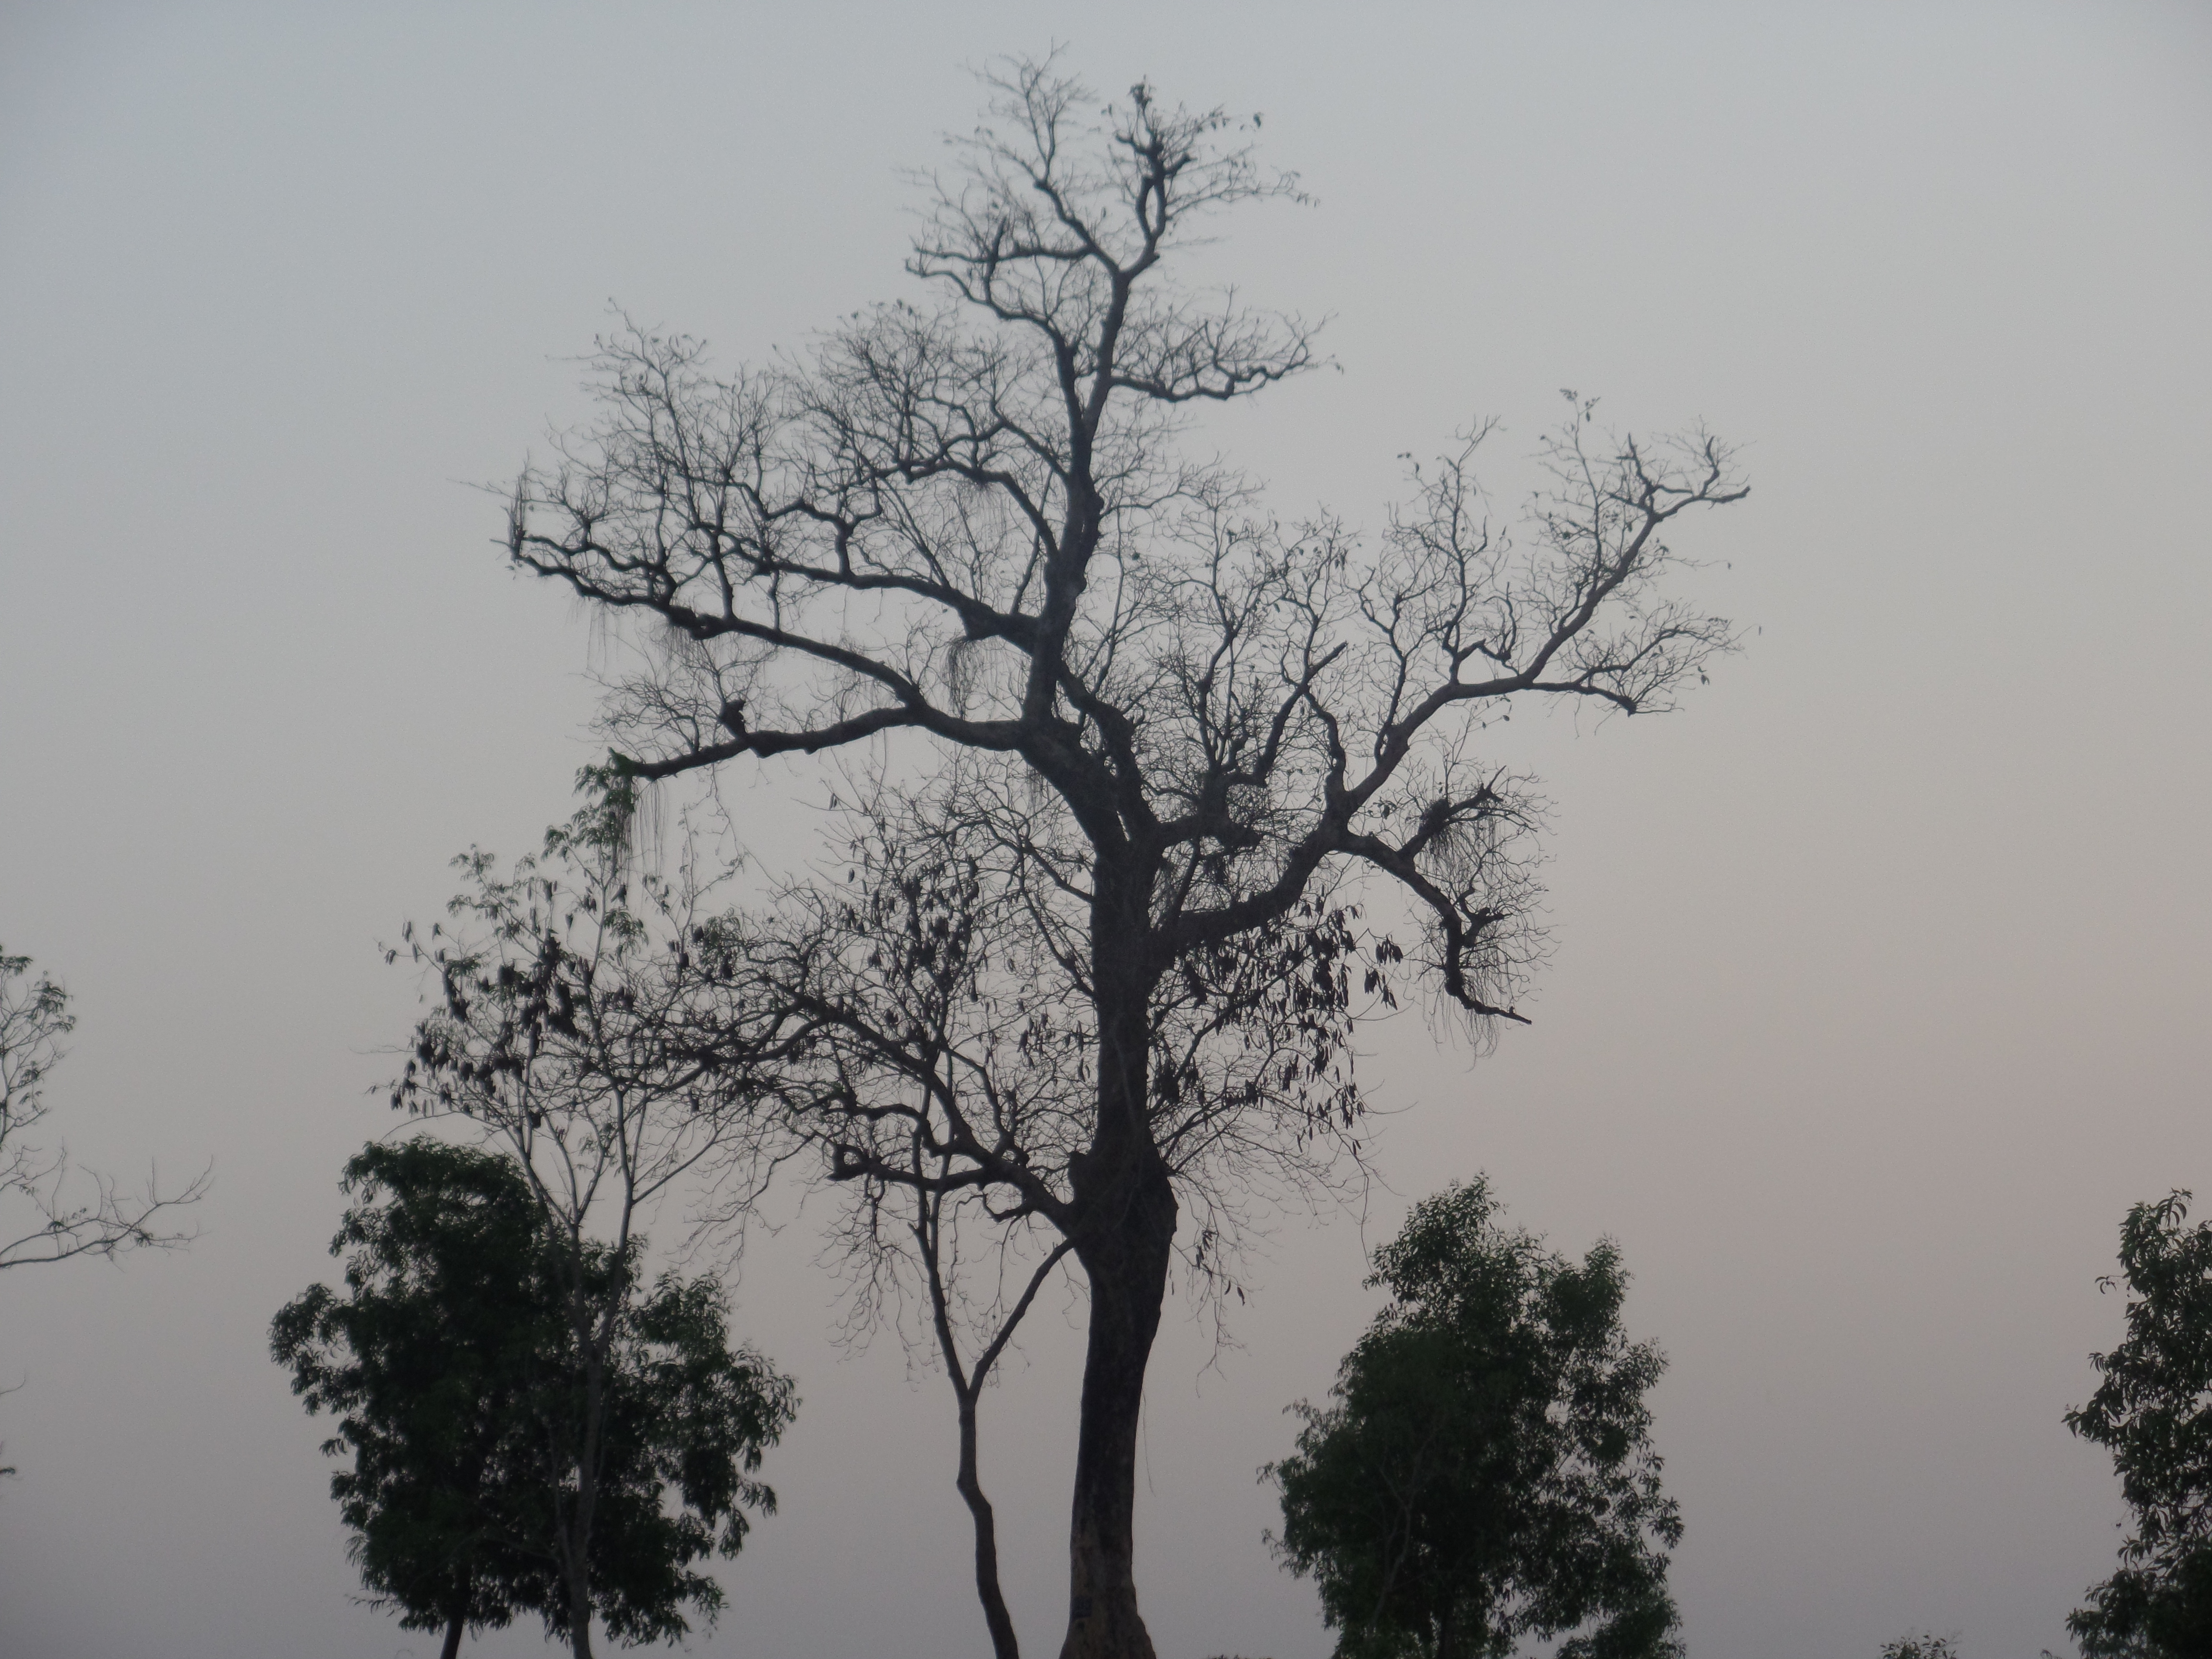
\includegraphics[width=0.4\linewidth,keepaspectratio]{tree}
\end{center}
Sample grammar rules:
\begin{center}
\includegraphics[width=0.4\linewidth,keepaspectratio]{grammar}
\end{center}
\end{frame}

%%%%%%%%%%%%%%%%%%%%%%%%%%%%%%%%%%%%%%%%%%%%%%%%%%%%%%%%%%%%%%%%%%%%%%%%%%%%%%%%%%
\begin{frame}[fragile]\frametitle{Core NLP Tasks: Named Entity Recognition}
\textbf{NER}: Identify and classify named entities
\begin{center}
\includegraphics[width=0.8\linewidth,keepaspectratio]{ner}
\end{center}

Common entity types:
\begin{itemize}
\item PERSON, ORGANIZATION, LOCATION
\item DATE, TIME, MONEY
\item PRODUCT, EVENT
\end{itemize}

Modern approaches: BERT-based models, few-shot learning with LLMs
\end{frame}

%%%%%%%%%%%%%%%%%%%%%%%%%%%%%%%%%%%%%%%%%%%%%%%%%%%%%%%%%%%%%%%%%%%%%%%%%%%%%%%%%%
\begin{frame}[fragile]\frametitle{Embedding}
\begin{center}
\includegraphics[width=0.6\linewidth,keepaspectratio]{nlpgoal}
\end{center}
\begin{itemize}
\item Convert letters, words, and ideas into numbers
\item Once we have numbers, we can use mathematics and machine learning
\item Humans like words, computers like numbers
\end{itemize}
\end{frame}

%%%%%%%%%%%%%%%%%%%%%%%%%%%%%%%%%%%%%%%%%%%%%%%%%%%%%%%%%%%%%%%%%%%%%%%%%%%%%%%%%%
\begin{frame}[fragile]\frametitle{Word Representations: The Evolution}
\textbf{Traditional: One-Hot Encoding}
\begin{itemize}
\item $Apple = [1, 0, 0, 0, ..., 0]$
\item $Orange = [0, 1, 0, 0, ..., 0]$
\item Problems: Sparse, no semantic meaning, huge dimensionality
\end{itemize}

\textbf{Modern: Dense Embeddings (Word2Vec, GloVe)}
\begin{itemize}
\item Each word → dense vector (e.g., 300 dimensions)
\item Similar words have similar vectors
\item $king - man + woman \approx queen$
\end{itemize}

\textbf{Latest: Contextual Embeddings (BERT, GPT)}
\begin{itemize}
\item Same word, different contexts → different vectors
\item "bank" in "river bank" vs "savings bank"
\item Captures polysemy and context
\end{itemize}
\end{frame}

%%%%%%%%%%%%%%%%%%%%%%%%%%%%%%%%%%%%%%%%%%%%%%%%%%%%%%%%%%%%%%%%%%%%%%%%%%%%%%%%%%
\begin{frame}[fragile]\frametitle{Word2Vec: Distributed Representations}
\begin{center}
\includegraphics[width=0.8\linewidth,keepaspectratio]{word41}
\end{center}

Key properties:
\begin{itemize}
\item Dense vectors (typically 100-300 dimensions)
\item Trained on large corpora (unsupervised)
\item Captures semantic relationships
\item Two architectures: CBOW, Skip-gram
\end{itemize}
\end{frame}

%%%%%%%%%%%%%%%%%%%%%%%%%%%%%%%%%%%%%%%%%%%%%%%%%%%%%%%%%%%%%%%%%%%%%%%%%%%%%%%%%%
\begin{frame}[fragile]\frametitle{Word Embeddings: Semantic Relationships}
Gender relation:
\begin{center}
\includegraphics[width=0.25\linewidth,keepaspectratio]{word45}
\end{center}

Country-capital relation:
\begin{center}
\includegraphics[width=0.4\linewidth,keepaspectratio]{word48}
\end{center}

Vector arithmetic captures analogies!
\end{frame}

%%%%%%%%%%%%%%%%%%%%%%%%%%%%%%%%%%%%%%%%%%%%%%%%%%%%%%%%%%%%%%%%%%%%%%%%%%%%%%%%%%
\begin{frame}[fragile]\frametitle{}
\begin{center}
{\Large NLP Applications}
\end{center}
\end{frame}

%%%%%%%%%%%%%%%%%%%%%%%%%%%%%%%%%%%%%%%%%%%%%%%%%%%%%%%%%%%%%%%%%%%%%%%%%%%%%%%%%%
\begin{frame}[fragile]\frametitle{NLP Applications: Text Classification}
\textbf{Text Categorization}: Assign predefined categories
\begin{center}
\includegraphics[width=0.8\linewidth,keepaspectratio]{textcat}
\end{center}

Applications:
\begin{itemize}
\item Spam detection
\item Sentiment analysis
\item Topic classification
\item Intent detection
\end{itemize}
\end{frame}

%%%%%%%%%%%%%%%%%%%%%%%%%%%%%%%%%%%%%%%%%%%%%%%%%%%%%%%%%%%%%%%%%%%%%%%%%%%%%%%%%%
\begin{frame}[fragile]\frametitle{NLP Applications: Sentiment Analysis}
\textbf{Sentiment Analysis}: Identify opinions and emotions
\begin{center}
\includegraphics[width=\linewidth,keepaspectratio]{sent}
\end{center}

Use cases:
\begin{itemize}
\item Product reviews
\item Social media monitoring
\item Customer feedback analysis
\item Financial market sentiment
\end{itemize}
\end{frame}

%%%%%%%%%%%%%%%%%%%%%%%%%%%%%%%%%%%%%%%%%%%%%%%%%%%%%%%%%%%%%%%%%%%%%%%%%%%%%%%%%%
\begin{frame}[fragile]\frametitle{Sentiment Analysis in Finance}
\begin{center}
\includegraphics[width=0.8\linewidth,keepaspectratio]{finnlp}
\end{center}

Applications:
\begin{itemize}
\item Stock market prediction
\item News impact analysis
\item Earnings call sentiment
\item Social media financial sentiment
\end{itemize}
\end{frame}

%%%%%%%%%%%%%%%%%%%%%%%%%%%%%%%%%%%%%%%%%%%%%%%%%%%%%%%%%%%%%%%%%%%%%%%%%%%%%%%%%%
\begin{frame}[fragile]\frametitle{NLP Applications: Information Retrieval}
\textbf{Information Retrieval}: Find relevant information
\begin{center}
\includegraphics[width=0.6\linewidth,keepaspectratio]{ie}
\end{center}

Components:
\begin{itemize}
\item Query understanding
\item Document ranking
\item Semantic search (beyond keyword matching)
\item Modern: Dense retrieval with embeddings
\end{itemize}
\end{frame}

%%%%%%%%%%%%%%%%%%%%%%%%%%%%%%%%%%%%%%%%%%%%%%%%%%%%%%%%%%%%%%%%%%%%%%%%%%%%%%%%%%
\begin{frame}[fragile]\frametitle{NLP Applications: Information Extraction}
\textbf{Information Extraction}: Extract structured information
\begin{center}
\includegraphics[width=0.6\linewidth,keepaspectratio]{iewiki}
\end{center}

Tasks:
\begin{itemize}
\item Named Entity Recognition
\item Relation Extraction
\item Event Extraction
\item Template Filling
\end{itemize}
\end{frame}

%%%%%%%%%%%%%%%%%%%%%%%%%%%%%%%%%%%%%%%%%%%%%%%%%%%%%%%%%%%%%%%%%%%%%%%%%%%%%%%%%%
\begin{frame}[fragile]\frametitle{NLP Applications: Machine Translation}
\textbf{Machine Translation}: Translate between languages
\begin{center}
\includegraphics[width=\linewidth,keepaspectratio]{trans}
\end{center}

Evolution:
\begin{itemize}
\item Rule-based MT (1950s-1980s)
\item Statistical MT (1990s-2010s)
\item Neural MT (2014-present)
\item Transformer-based (2017-present): Google Translate, DeepL
\end{itemize}
\end{frame}

%%%%%%%%%%%%%%%%%%%%%%%%%%%%%%%%%%%%%%%%%%%%%%%%%%%%%%%%%%%%%%%%%%%%%%%%%%%%%%%%%%
\begin{frame}[fragile]\frametitle{NLP Applications: Question Answering}
\textbf{Question Answering}: Provide direct answers to questions
\begin{center}
\includegraphics[width=0.6\linewidth,keepaspectratio]{start}
\end{center}

IBM Watson in Jeopardy (2011):
\begin{center}
\includegraphics[width=0.6\linewidth,keepaspectratio]{jeopardy}
\end{center}
\end{frame}

%%%%%%%%%%%%%%%%%%%%%%%%%%%%%%%%%%%%%%%%%%%%%%%%%%%%%%%%%%%%%%%%%%%%%%%%%%%%%%%%%%
\begin{frame}[fragile]\frametitle{NLP Applications: Text Summarization}
\textbf{Summarization}: Generate concise summaries
\begin{center}
\includegraphics[width=0.8\linewidth,keepaspectratio]{summry}
\end{center}

Types:
\begin{itemize}
\item Extractive: Select important sentences
\item Abstractive: Generate new summary text
\item Query-focused: Summarize w.r.t. specific query
\item Modern: Transformer-based abstractive (BART, T5, GPT)
\end{itemize}
\end{frame}

%%%%%%%%%%%%%%%%%%%%%%%%%%%%%%%%%%%%%%%%%%%%%%%%%%%%%%%%%%%%%%%%%%%%%%%%%%%%%%%%%%
\begin{frame}[fragile]\frametitle{NLP Applications: Topic Modeling}
\textbf{Topic Modeling}: Discover abstract topics in documents
\begin{center}
\includegraphics[width=0.6\linewidth,keepaspectratio]{topic}
\end{center}

Methods:
\begin{itemize}
\item Latent Dirichlet Allocation (LDA)
\item Non-negative Matrix Factorization (NMF)
\item BERTopic (modern approach)
\end{itemize}
\end{frame}

%%%%%%%%%%%%%%%%%%%%%%%%%%%%%%%%%%%%%%%%%%%%%%%%%%%%%%%%%%%%%%%%%%%%%%%%%%%%%%%%%%
\begin{frame}[fragile]\frametitle{NLP Applications: Modern Capabilities}
\textbf{Recent Breakthroughs with Large Language Models}:
\begin{itemize}
\item Code generation (GitHub Copilot, GPT-4)
\item Creative writing (stories, poems, scripts)
\item Conversational AI (ChatGPT, Claude, Gemini)
\item Multimodal understanding (text + images)
\item Reasoning and problem-solving
\item Few-shot and zero-shot learning
\end{itemize}

The field is rapidly evolving!
\end{frame}

%%%%%%%%%%%%%%%%%%%%%%%%%%%%%%%%%%%%%%%%%%%%%%%%%%%%%%%%%%%%%%%%%%%%%%%%%%%%%%%%%%
\begin{frame}[fragile]\frametitle{Modern NLP Stack (2025)}
\textbf{Foundation Models}:
\begin{itemize}
\item GPT-4, GPT-4o (OpenAI)
\item Claude 3.5 Sonnet, Claude 4 (Anthropic)
\item Gemini 1.5, Gemini 2.0 (Google)
\item LLaMA 3 (Meta)
\item Mistral, Mixtral (Mistral AI)
\end{itemize}

\textbf{Key Technologies}:
\begin{itemize}
\item Transformers with billions/trillions of parameters
\item Retrieval-Augmented Generation (RAG)
\item Reinforcement Learning from Human Feedback (RLHF)
\item Constitutional AI and alignment techniques
\item Multimodal architectures
\end{itemize}
\end{frame}

%%%%%%%%%%%%%%%%%%%%%%%%%%%%%%%%%%%%%%%%%%%%%%%%%%%%%%%%%%%%%%%%%%%%%%%%%%%%%%%%%%
\begin{frame}[fragile]\frametitle{Spell and Grammar Checking}
\begin{center}
\includegraphics[width=\linewidth,keepaspectratio]{spell}
\end{center}

Tasks:
\begin{itemize}
\item Spelling error detection and correction
\item Grammar error detection
\item Style suggestions
\item Modern: Context-aware corrections with LLMs
\end{itemize}
\end{frame}

%%%%%%%%%%%%%%%%%%%%%%%%%%%%%%%%%%%%%%%%%%%%%%%%%%%%%%%%%%%%%%%%%%%%%%%%%%%%%%%%%%
\begin{frame}[fragile]\frametitle{Word Prediction and Autocomplete}
\textbf{Word Prediction}: Predict next likely word
\begin{center}
\includegraphics[width=\linewidth,keepaspectratio]{wordpred}
\end{center}

Applications:
\begin{itemize}
\item Mobile keyboard typing
\item Search engine suggestions
\item Email composition
\item Code completion
\end{itemize}
\end{frame}

%%%%%%%%%%%%%%%%%%%%%%%%%%%%%%%%%%%%%%%%%%%%%%%%%%%%%%%%%%%%%%%%%%%%%%%%%%%%%%%%%%
\begin{frame}[fragile]\frametitle{Current State of NLP}
\begin{center}
\includegraphics[width=0.6\linewidth,keepaspectratio]{nlpstands}
\end{center}

NLP is embedded everywhere:
\begin{itemize}
\item Search engines
\item Virtual assistants
\item Customer service
\item Content moderation
\item Healthcare (clinical NLP)
\item Legal (contract analysis)
\end{itemize}
\end{frame}

%%%%%%%%%%%%%%%%%%%%%%%%%%%%%%%%%%%%%%%%%%%%%%%%%%%%%%%%%%%%%%%%%%%%%%%%%%%%%%%%%%
\begin{frame}[fragile]\frametitle{Level of Difficulty: Task Classification}
\textbf{Mostly Solved}:
\begin{itemize}
\item Spell checking and grammar correction
\item Part-of-speech tagging
\item Named entity recognition (common entities)
\item Basic text classification
\end{itemize}

\textbf{Good Progress}:
\begin{itemize}
\item Machine translation
\item Sentiment analysis
\item Information retrieval
\item Information extraction
\item Text summarization
\end{itemize}

\textbf{Still Challenging}:
\begin{itemize}
\item Complex reasoning and inference
\item Common sense understanding
\item Long-form coherent generation
\item Multilingual low-resource languages
\item Factual consistency and hallucination control
\end{itemize}
\end{frame}


%%%%%%%%%%%%%%%%%%%%%%%%%%%%%%%%%%%%%%%%%%%%%%%%%%%%%%%%%%%%%%%%%%%%%%%%%%%%%%%%%%
\begin{frame}[fragile]\frametitle{NLP Trends in 2025}
Trends driving NLP adoption:
\begin{itemize}
\item Enormous amount of machine-readable text
\begin{itemize}
\item Newspapers, web pages, social media
\item Medical records, financial filings
\item Product reviews, discussion forums
\end{itemize}
\item Conversational agents as primary interface
\begin{itemize}
\item ChatGPT, Claude, virtual assistants
\end{itemize}
\item Human-human interaction mediated by computers
\begin{itemize}
\item Social media, messaging platforms
\end{itemize}
\end{itemize}

This means copious data available for NLP system development!
\end{frame}

%%%%%%%%%%%%%%%%%%%%%%%%%%%%%%%%%%%%%%%%%%%%%%%%%%%%%%%%%%%%%%%%%%%%%%%%%%%%%%%%%%
\begin{frame}[fragile]\frametitle{The Promise of NLP}
Growing importance in multiple arenas:
\begin{itemize}
\item Scientific: accelerating research
\item Economic: business intelligence, automation
\item Social: breaking language barriers
\item Cultural: preserving and translating heritage
\end{itemize}

Wide range of stakeholders need NLP knowledge:
\begin{itemize}
\item Academia: linguistics, computer science, AI
\item Industry: HCI, business analysis, web development
\item Healthcare: clinical documentation, diagnosis support
\item Legal: contract analysis, legal research
\end{itemize}

Goal: Open NLP to a broad audience
\end{frame}

%%%%%%%%%%%%%%%%%%%%%%%%%%%%%%%%%%%%%%%%%%%%%%%%%%%%%%%%%%%%%%%%%%%%%%%%%%%%%%%%%%
\begin{frame}[fragile]\frametitle{NLP and Intelligence}
\begin{itemize}
\item Long-standing challenge: build intelligent machines
\item Chief measure of machine intelligence: linguistic capability
\item Turing Test: conversational ability as intelligence criterion
\end{itemize}

Example human-machine dialog:
\small
\begin{tabular}{ll}
S: & How may I help you?\\
U: & When is Saving Private Ryan playing?\\
S: & For what theater?\\
U: & The Paramount theater.\\
S: & Saving Private Ryan is not playing at the Paramount theater,\\
   & but it's playing at the Madison theater at 3:00, 5:30, and 10:30.
\end{tabular}
\end{frame}

%%%%%%%%%%%%%%%%%%%%%%%%%%%%%%%%%%%%%%%%%%%%%%%%%%%%%%%%%%%%%%%%%%%%%%%%%%%%%%%%%%
\begin{frame}[fragile]\frametitle{Current Limitations}
Today's systems limited to narrow domains:
\begin{itemize}
\item Can't easily add new capabilities
\item Require domain-specific training
\item Common-sense reasoning still challenging
\item Hallucination and factual errors
\item Lack of true understanding vs pattern matching
\end{itemize}

To improve, we need:
\begin{itemize}
\item Better knowledge representation
\item Improved reasoning capabilities
\item More robust grounding in reality
\item Continued research in alignment and safety
\end{itemize}
\end{frame}

%%%%%%%%%%%%%%%%%%%%%%%%%%%%%%%%%%%%%%%%%%%%%%%%%%%%%%%%%%%%%%%%%%%%%%%%%%%%%%%%%%
\begin{frame}[fragile]\frametitle{}
\begin{center}
{\Large Conclusion \& Outlook}
\end{center}
\end{frame}

%%%%%%%%%%%%%%%%%%%%%%%%%%%%%%%%%%%%%%%%%%%%%%%%%%%%%%%%%%%%%%%%%%%%%%%%%%%%%%%%%%
\begin{frame}[fragile]\frametitle{Key Takeaways}
\begin{itemize}
\item NLP is about making computers understand and generate human language
\item Language is inherently ambiguous and context-dependent
\item Multiple approaches: rules, ML, deep learning, LLMs
\item Huge progress in recent years, but challenges remain
\item Applications everywhere: search, translation, assistants, analysis
\end{itemize}

\begin{center}
\includegraphics[width=0.4\linewidth,keepaspectratio]{nlp_overview}
\end{center}
\end{frame}

%%%%%%%%%%%%%%%%%%%%%%%%%%%%%%%%%%%%%%%%%%%%%%%%%%%%%%%%%%%%%%%%%%%%%%%%%%%%%%%%%%
\begin{frame}[fragile]\frametitle{In Nutshell}
\begin{itemize}
\item NLP is an effort to do useful things with natural language
\item Humans like words, computers like numbers
\item We bridge this gap through representation learning
\item Modern NLP combines:
\begin{itemize}
\item Large data
\item Powerful compute
\item Advanced algorithms (Transformers, LLMs)
\end{itemize}
\item Exciting time to be in NLP - rapid innovation!
\end{itemize}
\end{frame}

%%%%%%%%%%%%%%%%%%%%%%%%%%%%%%%%%%%%%%%%%%%%%%%%%%%%%%%%%%%%%%%%%%%%%%%%%%%%%%%%%%
\begin{frame}[fragile]\frametitle{Resources and Next Steps}
\textbf{Learn More}:
\begin{itemize}
\item Stanford CS224N: Natural Language Processing with Deep Learning
\item fast.ai NLP course
\item Hugging Face tutorials and documentation
\item Papers: arxiv.org/list/cs.CL (Computation and Language)
\end{itemize}

\textbf{Practice}:
\begin{itemize}
\item Kaggle NLP competitions
\item Build projects with Hugging Face Transformers
\item Experiment with OpenAI API, Anthropic Claude
\item Contribute to open-source NLP libraries
\end{itemize}
\end{frame}

